%=== CHAPTER TWO (2) ===
%=== Literature Review ===

\chapter{Literature Review}
\begin{spacing}{1.5}
\setlength{\parskip}{0.3in}

% \section{Overview}
In this chapter, the definition and physiological features of skin pigmentation are first reviewed. Then, the field of computer graphics is examined, discussing how to model skin and pigmentation to achieve realistic skin image rendering. Finally, attention is turned to the field of computer vision, where state-of-the-art image modeling and editing methods are reviewed, assessing the degree of fit and gaps between the goals of this task and existing methods.

\section{Skin Chromophores \& Pigmentation}
\begin{figure}
    \centering
    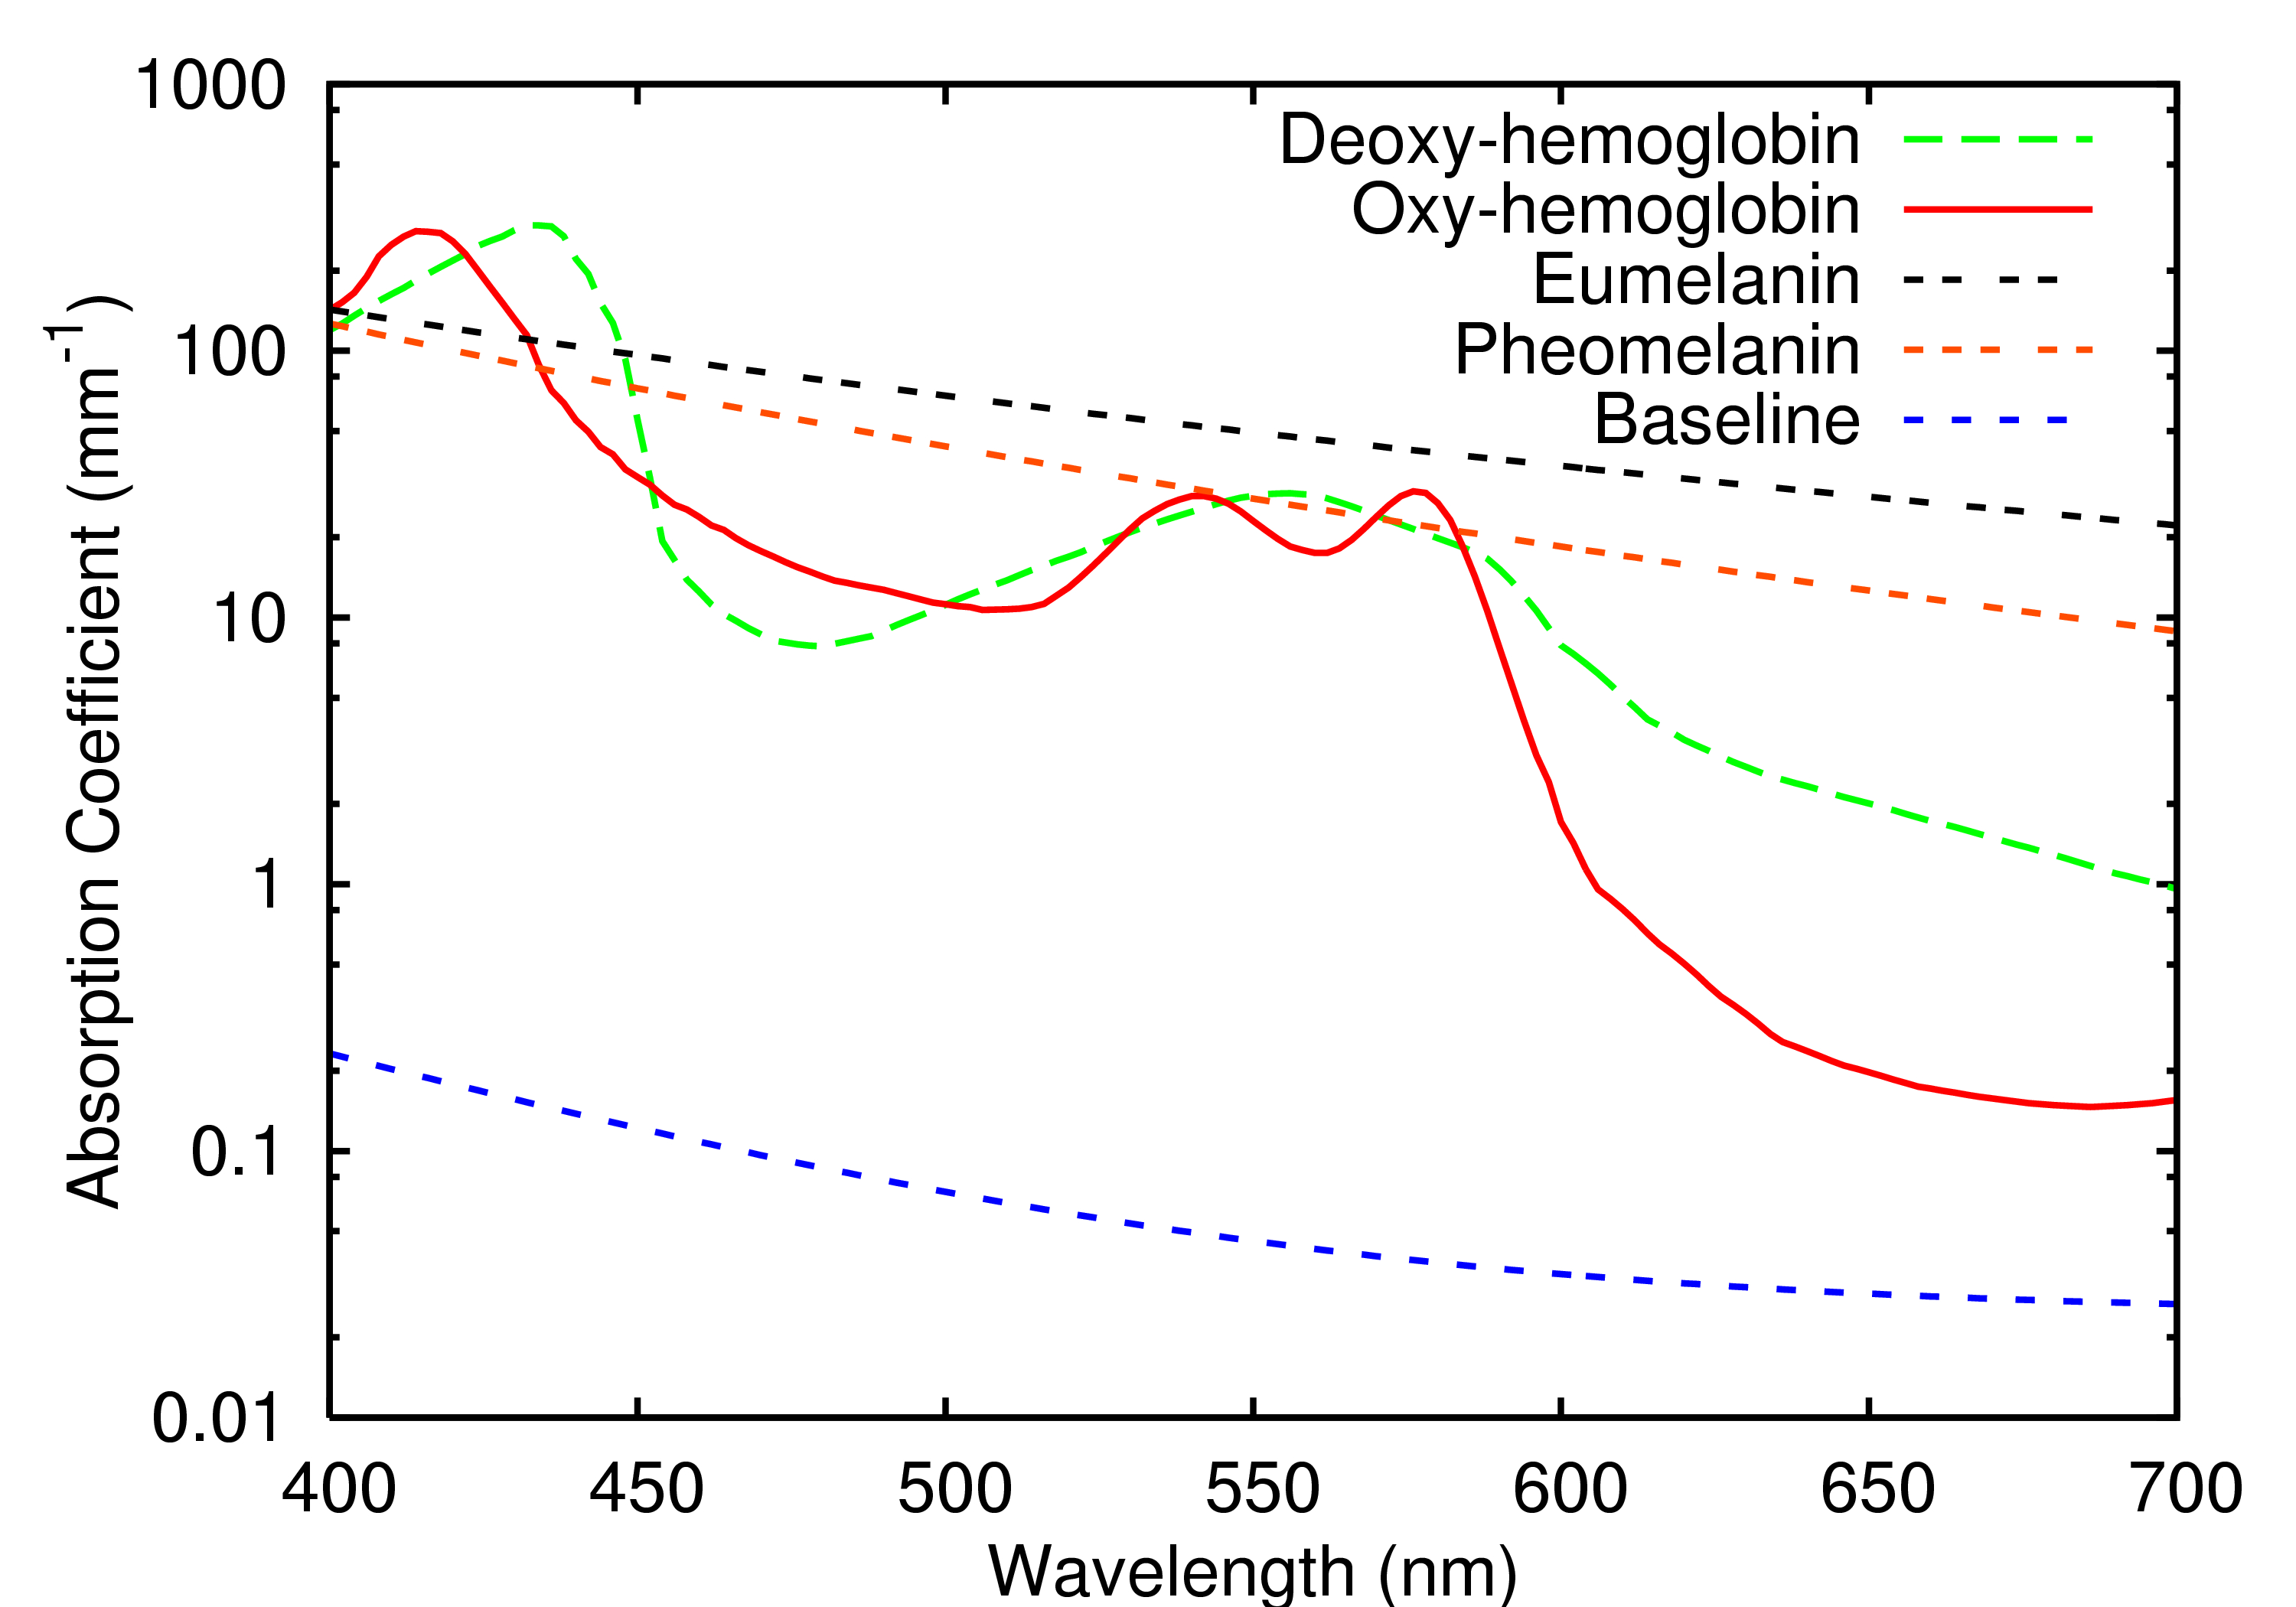
\includegraphics[width=0.9\columnwidth]{Chapter2/HM_abs.png}
    \caption{Spectral absorption coefficients of skin chromophore. This work focused on modelling heamoglobin and melanin distribution of skin pigmentation. Image taken from\cite{10.5555/2383894.2383946}}.
    \label{fig:hm_abs}
\end{figure}

What gives human skin its diverse colors? When light is transmitted into the skin, energy of different wavelengths is selectively absorbed by the chromophores, scattered by the skin tissues and then observed in unique colors. The color of human skin and skin pigmentations is primarily influenced by several key chromophores, namely \textit{Melanin}, \textit{Hemoglobin}, \textit{Carotene}, and \textit{Bilirubin}. These pigments, each with unique optical properties, contribute to the skin's overall coloration and appearance:

\begin{itemize}
    \item \textbf{Hemoglobin} Found in red blood cells, Hemoglobin gives blood its red color. The optical properties of Hemoglobin vary between its two forms: oxy-Hemoglobin (oxygen-rich) and deoxy-Hemoglobin (oxygen-poor). These forms have distinct absorption peaks in the visible spectrum, contributing to the reddish undertones of skin.
    \item \textbf{Melanin} Rather than being a singular entity, Melanin is a composite of various polymers, exhibiting a spectrum of shades ranging from pale yellow to deep brown or black. The lighter variants of melanin predominantly consist of \textit{pheomelanin}, whereas \textit{eumelanin} typically constitutes the darker forms of melanin\cite{alalufEthnicVariationMelanin2002a}. This is the primary determinant of skin color\cite{doiSpectralEstimationHuman2003}, providing shades from light to dark. Melanin absorbs across a broad range of the visible spectrum but particularly in the ultraviolet (UV) region\cite{ANDERSON198113}. This absorption is crucial as it protects the skin from UV radiation damage. 
    \item \textbf{Carotene and Bilirubin} These pigments impart a yellowish hue to the skin. They absorb light in the blue region of the spectrum, which complements the reds of Hemoglobin and the browns of melanin, contributing to the overall skin tone\cite{ANDERSON198113}.
\end{itemize}


In this work, mainly hemoglobin and melanin in the skin are considered. For the other chromophores and their appearance, they are used as residual terms. In Figure\ref{fig:hm_abs}, the spectral absorption coefficients of these two key chromophores are shown. Both types of hemoglobin have high absorption coefficients from 400nm to 450nm and from 520nm to 600nm, giving the skin a pink color appearance. Melanin, on the other hand, absorbs UV and blue-violet more strongly, giving the skin a brown to black appearance.

The formation of skin pigmentations, such as brown spots or red spots, is often associated with an overproduction or uneven distribution of skin chromophores. These pigmentations can result from various factors, including genetic predisposition, hormonal changes, sun exposure, and aging. In response to UV radiation, Melanocytes (melanin-producing cells) increase their production of melanin as a protective mechanism, which can lead to localized darkening of the skin.

\section{Skin Modeling \& Rendering Techniques}

\begin{figure}[t]
    \centering
    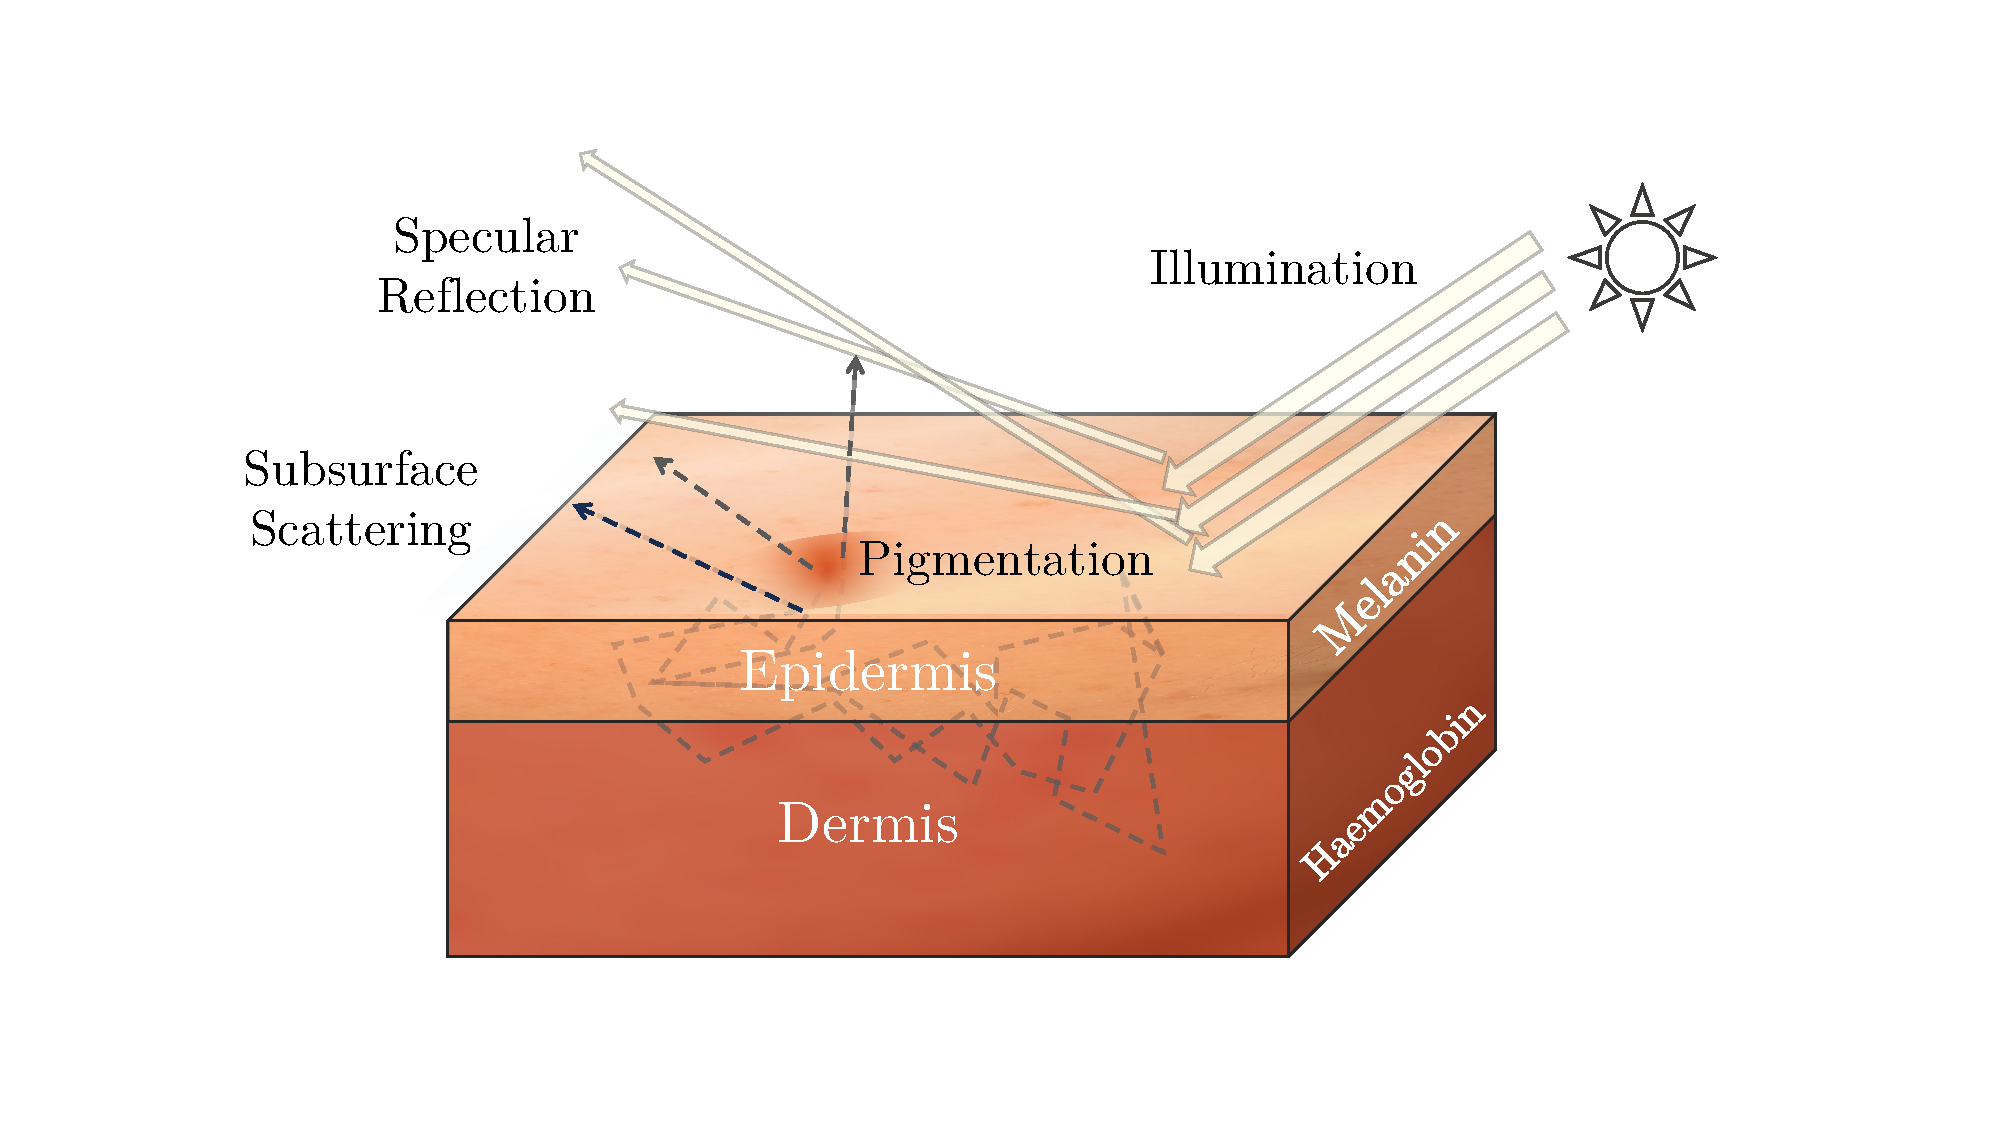
\includegraphics[width=0.9\columnwidth]{Chapter2/skin_model2.pdf}
    \caption{Layered skin model. A portion of the incident light undergoes specular reflection, revealed as a skin texture layer. The other part transmits into and is scattered by the Epidermis and Dermis. Melanin and haemoglobin, which are distributed in these two layers, absorb specific wavelengths of light, rendering the skin's characteristic color.}
    \label{fig:skin_model}
\end{figure}

Modeling skin as a layered, semi-transparent material has become common practice in studying the optical properties of skin and realistic skin rendering\cite{10.5555/2383894.2383946}. In this model, the interactions of light with the skin can be thought of as combinations of the following:

\begin{enumerate}
    \item \textbf{Specular reflection:} Light reflection from the surface, caused by oils, water, and stratum corneum of the skin. It captures the surface texture of the skin, such as fine grooves and textures. The proposed method preserves these details unaltered.
    \item \textbf{Subsurface scattering and absorption:} Physiologically, skin is semi-transparent\cite{Igarashi2005TheAO}. Skin constituents such as extra-cellular matrix cause random deflections of incoming light rays, some of which are reflected back to the surface and are observed. This phenomenon is called subsurface scattering. In addition, the chromophore components present in the epidermis and dermis layers, such as melanin and heamoglobin, selectively absorb light propagating in the skin, thus rendering the unique hue of human skin. When chromophore is locally accumulated, it will render a blemish where the color is different from the surrounding skin\cite{ANDERSON198113}. The proposed method emphasizes this unique optical phenomenon to achieve realistic pigmentation modelling and editing.
    \item \textbf{Transmission:} When the light is very strong and shines on thin tissue (such as the ears or fingers under strong light), a unique transmission appearance can be observed against the light source. For blemish change modelling, this aspect is disregarded.
\end{enumerate}

Despite the multilayer skin model describing the unique appearance resulting from skin optical properties well and conforming to the physiological structure of real skin, rendering realistic skin images on a computer has been challenging. 

Thanks to advancements in modern graphics hardware and developments in computer graphics, realistic skin rendering can now be achieved\cite{10.1145/1198555.1198593, 2015ExtendingTD, JIMENEZ2015_CGF}. The key lies in achieving an accurate and efficient simulation of the subsurface scattering behavior of the skin. Although ray tracing and path tracing\cite{wrenninge2017path, chiang2016practical} are regarded as some of the most realistic approximations for the behaviors of light rays, these methods often require massive computations and can be difficult to apply to real-time scenarios, so approximate fast algorithms become the primary consideration. Jensen et al.\cite{10.1145/3596711.3596747} proposed the Bidirectional Surface Scattering Reflectance Distribution Function (BSSRDF) to approximate the light transmission function. Based on their observations and assumptions, in highly scattering media, light scattering tends to be isotropic, so the scattering distribution is only related to the distance from the incident point. Based on this assumption, Eugene et al.\cite{d2007efficient} proposed using a diffusion profile to describe this scattering distribution, thereby achieving efficient and realistic skin rendering. However, it is still challenging to accurately simulate the scattering of the multilayer skin model. Fortunately, Jensen et al.\cite{10.1145/1073204.1073308} pointed out that using the sum of 4 or more Gaussian functions to approximate the diffusion profile of the multi-layer skin model has been proven to be very effective in practice. Moreover, they calculated a set of well-fitted parameters and successfully simulated the diffusion distribution of the multi-layer skin model in the RGB domain.

These methods have inspired the work to take into account the optical properties of the skin in the proposed algorithm, thus achieving realistic blemish simulation.

% \section{Controllable Facial Image Editing}

% \subsection{Objectives and Definitions}

% Deep learning-based methods aim to learn a projection from latent noise to pixels\cite{goodfellowGenerativeAdversarialNetworks2014,DBLP:conf/nips/HoJA20,DBLP:journals/corr/KingmaW13}. Once successfully trained, control over the generated image can be achieved by editing in their latent spaces\cite{DBLP:journals/corr/abs-1812-04948, DBLP:journals/corr/abs-1907-10786}. Additionally, achieving precise and controllable latent editing requires either encoding control parameters into the input noise, modelled as conditional generation\cite{isolaImagetoimageTranslationConditional2017}, or injecting controls into the forward pipeline, such as Low-Rank Adaption(LoRA)\cite{2021arXiv210609685H} or ControlNet\cite{2023arXiv230205543Z}, etc. These methods all require calibrated and labelled data with model fine-tuning to achieve accurate editing.

% This physics-based modelling approach simulates the optical properties and physiological characteristics of the skin to model the relative distribution of localized skin chromophores. This is achieved through fitting the Sum-of-Gaussians. This method allows skin-agnostic control over the shape, color, and size of local skin blemishes to simulate their degradation or deterioration process after fitting. Without extensive training data, this method is comparable in effect to deep learning models, with strong interpretability.

% \subsection{Dataset and Stability}

% Deep learning-based approaches are highly dependent on dataset quality. On small datasets, deep neural networks are often prone to over-fitting, showing similar generation patterns or binding certain features to another (e.g., binding specific skin tone to a gender, or certain age range). Additionally, if there are not enough samples reflecting continuous changes in the same subject, it becomes challenging for the model to learn a trajectory that fits reality.

% On one hand, recent high-resolution portrait datasets\cite{DBLP:journals/corr/abs-1812-04948} have been proposed, facilitating deep learning models to achieve great success in face image generation. However, they mostly focus on coarse, large-scale features (such as face shape, hairstyle, expression, etc.). On the other hand, datasets for skin texture rendering\cite{Bai_2023_CVPR} have been proposed. But they generally contain “flawless” skin with few real skin texture samples reflecting skin diseases or defects, and there are no corresponding annotations. To the authors' knowledge, there is currently no dataset specifically dedicated to skin blemish generation or editing.

\section{Controllable Facial Image Editing}

\subsection{Objectives and Definitions}

Deep learning-based methods, notably Generative Adversarial Networks (GANs) and Diffusion models, have been instrumental in image content editing, learning a projection from latent noise to pixels \cite{goodfellowGenerativeAdversarialNetworks2014,DBLP:conf/nips/HoJA20,DBLP:journals/corr/KingmaW13}. Control over the generated image in these methods is typically achieved through latent space manipulation \cite{DBLP:journals/corr/abs-1812-04948, DBLP:journals/corr/abs-1907-10786}. After training, additional precise control over these methods requires embedding control parameters within the input noise or the model's pipeline, often using techniques like Low-Rank Adaption (LoRA) \cite{2021arXiv210609685H} or ControlNet \cite{2023arXiv230205543Z}. However, these methods necessitate extensive data annotation and model fine-tuning for effective and accurate editing.

Contrastingly, this research adopts a physics-based modelling approach, which focuses on the optical and physiological properties of skin. By employing a Sum-of-Gaussians fitting, it facilitates control over the shape, color, and size of local skin blemishes. This approach simulates their natural degradation process, functioning effectively without extensive training datasets, thus offering an interpretability advantage over deep learning models.

\subsection{Dataset and Stability}

The efficacy of deep learning-based methods is heavily contingent on dataset quality. These models often suffer from overfitting on small datasets, leading to repetitive generation patterns or erroneous feature associations (e.g., linking specific skin tones to gender or age). Moreover, the absence of samples depicting gradual changes in the same subject hampers the model's ability to learn realistic trajectories.

Although recent advancements in high-resolution portrait datasets \cite{DBLP:journals/corr/abs-1812-04948} have propelled deep learning models in face image generation, these datasets primarily encompass coarse features like face shape and expression. Skin texture datasets, such as those proposed in Bai et al. \cite{Bai_2023_CVPR}, offer insights into skin rendering. However, they typically showcase near-perfect skin textures, lacking in representations of skin anomalies or diseases. Recent works have been explored for skin pigmentation generation\cite{beharaSkinLesionSynthesis2023} but lack explicit control over the output nor the ability to modify existing images.

In contrast, the proposed method introduces a novel physical-based model that operates independently of paired image datasets. This approach circumvents the limitations imposed by the lack of comprehensive and diverse data typical in deep learning frameworks. By modeling the optical and physiological characteristics of skin using a Sum-of-Gaussians approach, it enables the simulation of natural blemish fading processes with high fidelity. The independence from paired image datasets not only reduces the reliance on extensive data collection and annotation but also enhances the model's applicability to a broader range of scenarios and skin types, making it a significant advancement in the field of facial image editing.

\subsection{Controllability}
In this section, the categorization of image content editing methods into three distinct classes is presented: Pixel Space, Latent Space, and Parameter Space.

\begin{itemize}
    \item \textbf{Pixel Space}: This class includes methods operating at the pixel level, such as inpainting and filtering. Inpainting techniques use neighboring or similar pixels for blemish correction \cite{bertalmio2001navier, lipowezkyAutomaticFrecklesDetection2008, Liu2017AutomaticFF}. However, these approaches often result in unnatural editing due to simplistic interpolation and blemish pixel detection via hard thresholding. Filtering methods apply content-aware smoothing to maintain skin details while removing blemishes \cite{velusamyFabSoftenFaceBeautification2020, heGuidedImageFiltering2010}, but they do not fully address the gradual fading of blemishes.

    \item \textbf{Latent Space}: Deep generative models, such as those proposed by Goodfellow et al. and Rombach et al., map latent noise to pixels \cite{goodfellowGenerativeAdversarialNetworks2014,rombach2021highresolution}. This approach, termed latent space editing, has been applied in skin pigmentation generation and face image retouching \cite{beharaSkinLesionSynthesis2023, xieBlemishawareProgressiveFace2023, liuAutomaticBeautificationGroupPhoto2018}. While these models facilitate smooth image transitions, they often lack explicit control for modifying existing images.

    \item \textbf{Parameter Space}: Referred to as Parametric Space editing, this category involves physics-based methods that model skin optics and physiology. By adjusting model parameters, facial image modification is achieved \cite{jungDeepLearningbasedOptical2023a, tsumuraImagebasedSkinColor}. Lin et al. introduced a method for modifying chromophore content in pigmentation, focusing on holistic adjustments \cite{linExemplarbasedFreckleRetouching2019}.

\end{itemize}

The proposed method introduces an innovative physical-based model enabling precise, per-spot chromophore concentration modeling and retouching without relying on paired image datasets. This approach, utilizing logarithmic RGB space decomposition, more accurately represents chromophore light absorption. It accounts for blurred blemish edges due to subsurface scattering, enabling seamless integration with the surrounding skin. This method stands out for its unprecedented control over blemish modifications attributed to localized chromophore accumulation, marking a novel advancement in this field.

%=== END OF CHAPTER TWO ===
\end{spacing}
\newpage
